\documentclass[output=paper,newtxmath,modfonts,nonflat,final]{langsci/langscibook} 
\ChapterDOI{10.5281/zenodo.3367148}
\author{Emily Moeng\affiliation{University of North Carolina, Chapel Hill}\lastand William Carter\affiliation{University of North Carolina, Chapel Hill}}
\title{Factors in the affrication of the ejective alveolar fricative in Tigrinya}

\IfFileExists{../localcommands.tex}{%hack to check whether this is being compiled as part of a collection or standalone
  \usepackage{pifont}
\usepackage{savesym}

\savesymbol{downingtriple}
\savesymbol{downingdouble}
\savesymbol{downingquad}
\savesymbol{downingquint}
\savesymbol{suph}
\savesymbol{supj}
\savesymbol{supw}
\savesymbol{sups}
\savesymbol{ts}
\savesymbol{tS}
\savesymbol{devi}
\savesymbol{devu}
\savesymbol{devy}
\savesymbol{deva}
\savesymbol{N}
\savesymbol{Z}
\savesymbol{circled}
\savesymbol{sem}
\savesymbol{row}
\savesymbol{tipa}
\savesymbol{tableauxcounter}
\savesymbol{tabhead}
\savesymbol{inp}
\savesymbol{inpno}
\savesymbol{g}
\savesymbol{hanl}
\savesymbol{hanr}
\savesymbol{kuku}
\savesymbol{ip}
\savesymbol{lipm}
\savesymbol{ripm}
\savesymbol{lipn}
\savesymbol{ripn} 
% \usepackage{amsmath} 
% \usepackage{multicol}
\usepackage{qtree} 
\usepackage{tikz-qtree,tikz-qtree-compat}
% \usepackage{tikz}
\usepackage{upgreek}


%%%%%%%%%%%%%%%%%%%%%%%%%%%%%%%%%%%%%%%%%%%%%%%%%%%%
%%%                                              %%%
%%%           Examples                           %%%
%%%                                              %%%
%%%%%%%%%%%%%%%%%%%%%%%%%%%%%%%%%%%%%%%%%%%%%%%%%%%%
% remove the percentage signs in the following lines
% if your book makes use of linguistic examples
\usepackage{tipa}  
\usepackage{pstricks,pst-xkey,pst-asr}

%for sande et al
\usepackage{pst-jtree}
\usepackage{pst-node}
%\usepackage{savesym}


% \usepackage{subcaption}
\usepackage{multirow}  
\usepackage{./langsci/styles/langsci-optional} 
\usepackage{./langsci/styles/langsci-lgr} 
\usepackage{./langsci/styles/langsci-glyphs} 
\usepackage[normalem]{ulem}
%% if you want the source line of examples to be in italics, uncomment the following line
% \def\exfont{\it}
\usetikzlibrary{arrows.meta,topaths,trees}
\usepackage[linguistics]{forest}
\forestset{
	fairly nice empty nodes/.style={
		delay={where content={}{shape=coordinate,for parent={
					for children={anchor=north}}}{}}
}}
\usepackage{soul}
\usepackage{arydshln}
% \usepackage{subfloat}
\usepackage{langsci/styles/langsci-gb4e} 
   
% \usepackage{linguex}
\usepackage{vowel}

\usepackage{pifont}% http://ctan.org/pkg/pifont
\newcommand{\cmark}{\ding{51}}%
\newcommand{\xmark}{\ding{55}}%
 
 
 %Lamont
 \makeatletter
\g@addto@macro\@floatboxreset\centering
\makeatother

\usepackage{newfloat} 
\DeclareFloatingEnvironment[fileext=tbx,name=Tableau]{tableau}
  %add all your local new commands to this file
\newcommand{\downingquad}[4]{\parbox{2.5cm}{#1}\parbox{3.5cm}{#2}\parbox{2.5cm}{#3}\parbox{3.5cm}{#4}}
\newcommand{\downingtriple}[3]{\parbox{4.5cm}{#1}\parbox{3cm}{#2}\parbox{3cm}{#3}}
\newcommand{\downingdouble}[2]{\parbox{4.5cm}{#1}\parbox{6cm}{#2}}
\newcommand{\downingquint}[5]{\parbox{1.75cm}{#1}\parbox{2.25cm}{#2}\parbox{2cm}{#3}\parbox{3cm}{#4}\parbox{2cm}{#5}}
\newcolumntype{Y}{>{\centering\arraybackslash}X}
\newcolumntype{T}{>{\centering\arraybackslash}m{2cm}}

%commands for Kusmer paper below
\newcommand{\ip}{$\upiota$}
\newcommand{\lipm}{(\_{\ip-Max}}
\newcommand{\ripm}{)\_{\ip-Max}}
\newcommand{\lipn}{(\_{\ip}}
\newcommand{\ripn}{)\_{\ip}}
\renewcommand{\_}[1]{\textsubscript{#1}}


%commands for Pillion paper below
\newcommand{\suph}{\textipa{\super h}}
\newcommand{\supj}{\textipa{\super j}}
\newcommand{\supw}{\textipa{\super w}}
\newcommand{\ts}{\textipa{\t{ts}}}
\newcommand{\tS}{\textipa{\t{tS}}}
\newcommand{\devi}{\textipa{\r*i}}
\newcommand{\devu}{\textipa{\r*u}}
\newcommand{\devy}{\textipa{\r*y}}
\newcommand{\deva}{\textipa{\r*a}}
\renewcommand{\N}{\textipa{N}}
\newcommand{\Z}{\textipa{Z}}
% 

%commands for Diercks paper below
\newcommand{\circled}[1]{\begin{tikzpicture}[baseline=(word.base)]
\node[draw, rounded corners, text height=8pt, text depth=2pt, inner sep=2pt, outer sep=0pt, use as bounding box] (word) {#1};
\end{tikzpicture}
}

%commands for Pesetsky paper below
% \newcommand{\sem}[2][]{\mbox{$[\![ $\textbf{#2}$ ]\!]^{#1}$}}
\newcommand{\sem}[2][]{\mbox{$[[ $\textbf{#2}$ ]]^{#1}$}}

% \newcommand{\ripn}{{\color{red}ripn}}%this is used but never defined. Please update the definition



%commands for Lamont paper below
\newcommand{\row}[4]{
	#1. & 
    /{#2}/ & 
    [{#3}] & 
    `#4' \\ 
}
%\newcounter{tableauxcounter}
\newcommand{\tabhead}[2]{
%     \captionsetup{labelformat=empty}
%     \stepcounter{tableauxcounter}
%     \addtocounter{table}{-1}
% 	\centering
% 	\caption{Tableau \thetableauxcounter: #1}
	\caption{#1}
	\label{#2}
}
\newcommand{\candref}[2]{{(\ref{#1}#2)}}
\newcommand{\tableauref}[1]{{Tableau~\ref{#1}}}
% tableaux
\newcommand{\inp}[1]{\multicolumn{2}{|l||}{{#1}}}
\newcommand{\inpno}[1]{\multicolumn{2}{|l||}{#1}}
\newcommand{\g}{\cellcolor{lightgray}}
\newcommand{\hanl}{\HandLeft}
\newcommand{\hanr}{\HandRight}
\newcommand{\kuku}{Kuk\'{u}}

% \newcommand{\nocaption}[1]{{\color{red} Please provide a caption}}

% \providecommand{\biberror}[1]{{\color{red}#1}}

\definecolor{RED}{cmyk}{0.05,1,0.8,0}


\newfontfamily\amharicfont[Script = Ethiopic, Scale = 1.0]{AbyssinicaSIL}
\newcommand{\amh}[1]{{\amharicfont #1}}

% 
% %Gjersoe
\usepackage{textgreek}
% 
\newcommand{\viol}{\fontfamily{MinionPro-OsF}\selectfont\rotatebox{60}{$\star$}}
\newcommand{\myscalex}{0.45}
\newcommand{\myscaley}{0.65}
%\newcommand{\red}[1]{\textcolor{red}{#1}}
%\newcommand{\blue}[1]{\textcolor{blue}{#1}}
\newcommand{\epen}[1]{\colorbox{jgray}{#1}}
\newcommand{\hand}{{\normalsize \ding{43}}}
\definecolor{jgray}{gray}{0.8} 
\usetikzlibrary{positioning}
\usetikzlibrary{matrix}
\newcommand{\mora}{\textmu\xspace}
\newcommand{\si}{\textsigma\xspace}
\newcommand{\ft}{\textPhi\xspace}
\newcommand{\tone}{\texttau\xspace}
\newcommand{\word}{\textomega\xspace}
% \newcommand{\ts}{\texttslig}
\newcommand{\fns}{\footnotesize}
\newcommand{\ns}{\normalsize}
\newcommand{\vs}{\vspace{1em}}
\newcommand{\bs}{\textbackslash}   % backslash
\newcommand{\cmd}[1]{{\bf \color{red}#1}}   % highlights command
\newcommand{\scell}[2][l]{\begin{tabular}[#1]{@{}c@{}}#2\end{tabular}}
% \interfootnotelinepenalty=10000

% --- Snider Representations --- %

\newcommand{\RepLevelHh}{
\begin{minipage}{0.10\textwidth}
\begin{tikzpicture}[xscale=\myscalex,yscale=\myscaley]
%\node (syl) at (0,0) {Hi};
\node (Rt) at (0,1) {o};
\node (H) at (-0.5,2) {H};
\node (R) at (0.5,3) {h};
%\draw [thick] (syl.north) -- (Rt.south) ;
\draw [thick] (Rt.north) -- (H.south) ;
\draw [thick] (Rt.north) -- (R.south) ;
\end{tikzpicture}
\end{minipage}
}

\newcommand{\RepLevelLh}{
\begin{minipage}{0.10\textwidth}
\begin{tikzpicture}[xscale=\myscalex,yscale=\myscaley]
%\node (syl) at (0,0) {Mid2};
\node (Rt) at (0,1) {o};
\node (H) at (-0.5,2) {L};
\node (R) at (0.5,3) {h};
%\draw [thick] (syl.north) -- (Rt.south) ;
\draw [thick] (Rt.north) -- (H.south) ;
\draw [thick] (Rt.north) -- (R.south) ;
\end{tikzpicture}
\end{minipage}
}

\newcommand{\RepLevelHl}{
\begin{minipage}{0.10\textwidth}
\begin{tikzpicture}[xscale=\myscalex,yscale=\myscaley]
%\node (syl) at (0,0) {Mid1};
\node (Rt) at (0,1) {o};
\node (H) at (-0.5,2) {H};
\node (R) at (0.5,3) {l};
%\draw [thick] (syl.north) -- (Rt.south) ;
\draw [thick] (Rt.north) -- (H.south) ;
\draw [thick] (Rt.north) -- (R.south) ;
\end{tikzpicture}
\end{minipage}
}

\newcommand{\RepLevelLl}{
\begin{minipage}{0.10\textwidth}
\begin{tikzpicture}[xscale=\myscalex,yscale=\myscaley]
%\node (syl) at (0,0) {Lo};
\node (Rt) at (0,1) {o};
\node (H) at (-0.5,2) {L};
\node (R) at (0.5,3) {l};
%\draw [thick] (syl.north) -- (Rt.south) ;
\draw [thick] (Rt.north) -- (H.south) ;
\draw [thick] (Rt.north) -- (R.south) ;
\end{tikzpicture}
\end{minipage}
}

% --- Representations --- %

\newcommand{\RepLevel}{
\begin{minipage}{0.10\textwidth}
\begin{tikzpicture}[xscale=\myscalex,yscale=\myscaley]
\node (syl) at (0,0) {\textsigma};
\node (Rt) at (0,1) {o};
\node (H) at (-0.5,2) {\texttau};
\node (R) at (0.5,3) {\textrho};
\draw [thick] (syl.north) -- (Rt.south) ;
\draw [thick] (Rt.north) -- (H.south) ;
\draw [thick] (Rt.north) -- (R.south) ;
\end{tikzpicture}
\end{minipage}
}

\newcommand{\RepContour}{
\begin{minipage}{0.10\textwidth}
\begin{tikzpicture}[xscale=\myscalex,yscale=\myscaley]
\node (syl) at (0,0) {\textsigma};
\node (Rt) at (0,1) {o};
\node (H) at (-0.5,2) {\texttau};
\node (R) at (0.5,3) {\textrho};
\node (Rt2) at (1.5,1.0) {o};
%\node (H2) at (1.0,2) {$\tau$};
%\node (R2) at (2.0,2.5) {R};
\draw [thick] (syl.north) -- (Rt.south) ;
\draw [thick] (Rt.north) -- (H.south) ;
\draw [thick] (Rt.north) -- (R.south) ;
\draw [thick] (syl.north) -- (Rt2.south) ;
%\draw [thick] (Rt2.north) -- (H2.south) ;
%\draw [thick] (Rt2.north) -- (R2.south) ;
\end{tikzpicture}
\end{minipage}
}


% --- OT constraints --- %

\newcommand{\IllustrationDown}{
\begin{minipage}{0.09\textwidth}
\begin{tikzpicture}[xscale=0.7,yscale=0.45]
\node (reg) at (0,0.75) {{\small \textalpha}};
\node (arrow) at (0,0) {{\fns $\downarrow$}};
\node (Rt) at (0,-0.75) {{\small \textbeta}};
\end{tikzpicture}
\end{minipage}
}

\newcommand{\IllustrationUp}{
\begin{minipage}{0.09\textwidth}
\begin{tikzpicture}[xscale=0.7,yscale=0.45]
\node (reg) at (0,0.75) {{\small \textalpha}};
\node (arrow) at (0,0) {{\fns $\uparrow$}};
\node (Rt) at (0,-0.75) {{\small \textbeta}};
\end{tikzpicture}
\end{minipage}
}

\newcommand{\MaxAB}{
\begin{minipage}{0.09\textwidth}
\begin{tikzpicture}[xscale=0.6,yscale=0.4]
\node (max) at (0,0) {{\small \textsc{Max}}};
\node (reg) at (0.75,0.5) {{\fns \textalpha}};
\node (arrow) at (0.75,0) {{\tiny $\downarrow$}};
\node (Rt) at (0.75,-0.5) {{\fns \textbeta}};
\end{tikzpicture}
\end{minipage}
}

\newcommand{\DepAB}{
\begin{minipage}{0.09\textwidth}
\begin{tikzpicture}[xscale=0.6,yscale=0.4]
\node (max) at (0,0) {{\small \textsc{Dep}}};
\node (reg) at (0.75,0.5) {{\fns \textalpha}};
\node (arrow) at (0.75,0) {{\tiny $\downarrow$}};
\node (Rt) at (0.75,-0.5) {{\fns \textbeta}};
\end{tikzpicture}
\end{minipage}
}

\newcommand{\DepHReg}{
\begin{minipage}{0.055\textwidth}
\begin{tikzpicture}[xscale=0.6,yscale=0.4]
\node (dep) at (0,0) {{\small \textsc{Dep}}};
\node (reg) at (0,-1.0) {{\small h}};
\end{tikzpicture}
\end{minipage}
}

\newcommand{\DepLReg}{
\begin{minipage}{0.055\textwidth}
\begin{tikzpicture}[xscale=0.6,yscale=0.4]
\node (dep) at (0,0) {{\small \textsc{Dep}}};
\node (reg) at (0,-1.0) {{\small l}};
\end{tikzpicture}
\end{minipage}
}

\newcommand{\DepReg}{
\begin{minipage}{0.055\textwidth}
\begin{tikzpicture}[xscale=0.6,yscale=0.4]
\node (dep) at (0,0) {{\small \textsc{Dep}}};
\node (reg) at (0,-1.0) {{\small \textrho}};
\end{tikzpicture}
\end{minipage}
}

\newcommand{\DepTRt}{
\begin{minipage}{0.1\textwidth}
\begin{tikzpicture}[xscale=0.6,yscale=0.4]
\node (dep) at (0,0) {{\small \textsc{Dep}}};
\node (t) at (0.75,0.5) {{\fns \texttau}};
\node (arrow) at (0.75,0) {{\tiny $\downarrow$}};
\node (Rt) at (0.75,-0.5) {{\fns o}};
\end{tikzpicture}
\end{minipage}
}

\newcommand{\MaxRegRt}{
\begin{minipage}{0.1\textwidth}
\begin{tikzpicture}[xscale=0.6,yscale=0.4]
\node (max) at (0,0) {{\small \textsc{Max}}};
\node (arrow) at (0.75,0) {{\tiny $\downarrow$}};
\node (Rt) at (0.75,-0.5) {{\fns o}};
\node (reg) at (0.75,0.5) {{\fns \textrho}};
\end{tikzpicture}
\end{minipage}
}

\newcommand{\RegToneByRt}{
\begin{minipage}{0.06\textwidth}
\begin{tikzpicture}[xscale=0.6,yscale=0.5]
\node[rotate=20] (arrow1) at (-0.15,0) {{\fns $\uparrow$}};
\node[rotate=340] (arrow2) at (0.15,0) {{\fns $\uparrow$}};
\node (Rt) at (0,-0.55) {{\small o}};
\node (reg) at (0.4,0.55) {{\small \textrho}};
\node (tone) at (-0.4,0.55) {{\small \texttau}};
\end{tikzpicture}
\end{minipage}
}

\newcommand{\RegToneBySyl}{
\begin{minipage}{0.06\textwidth}
\begin{tikzpicture}[xscale=0.6,yscale=0.5]
\node[rotate=20] (arrow1) at (-0.15,0) {{\fns $\uparrow$}};
\node[rotate=340] (arrow2) at (0.15,0) {{\fns $\uparrow$}};
\node (Rt) at (0,-0.55) {{\small \textsigma}};
\node (reg) at (0.4,0.55) {{\small \textrho}};
\node (tone) at (-0.4,0.55) {{\small \texttau}};
\end{tikzpicture}
\end{minipage}
}

\newcommand{\DepTone}{
\begin{minipage}{0.055\textwidth}
\begin{tikzpicture}[xscale=0.6,yscale=0.4]
\node (dep) at (0,0) {{\small \textsc{Dep}}};
\node (tone) at (0,-1.0) {{\small \texttau}};
\end{tikzpicture}
\end{minipage}
}

\newcommand{\DepTonalRt}{
\begin{minipage}{0.055\textwidth}
\begin{tikzpicture}[xscale=0.6,yscale=0.4]
\node (dep) at (0,0) {{\small \textsc{Dep}}};
\node (tone) at (0,-1.0) {{\small o}};
\end{tikzpicture}
\end{minipage}
}

\newcommand{\DepL}{
\begin{minipage}{0.055\textwidth}
\begin{tikzpicture}[xscale=0.6,yscale=0.4]
\node (dep) at (0,0) {{\small \textsc{Dep}}};
\node (tone) at (0,-1.0) {{\small L}};
\end{tikzpicture}
\end{minipage}
}

\newcommand{\DepH}{
\begin{minipage}{0.055\textwidth}
\begin{tikzpicture}[xscale=0.6,yscale=0.4]
\node (dep) at (0,0) {{\small \textsc{Dep}}};
\node (tone) at (0,-1.0) {{\small H}};
\end{tikzpicture}
\end{minipage}
}

\newcommand{\NoMultDiff}{{\small *loh}}
\newcommand{\Alt}{{\small \textsc{Alt}}}
\newcommand{\NoSkip}{{\small \scell{\textsc{No}\\\textsc{Skip}}}}


\newcommand{\RegDomRt}{
\begin{minipage}{0.030\textwidth}
\begin{tikzpicture}[xscale=0.6,yscale=0.5]
\node (arrow) at (0,0) {{\fns $\downarrow$}};
\node (Rt) at (0,-0.55) {{\small o}};
\node (reg) at (0,0.55) {{\small \textrho}};
\end{tikzpicture}
\end{minipage}
}

\newcommand{\DepRegRt}{
\begin{minipage}{0.1\textwidth}
\begin{tikzpicture}[xscale=0.6,yscale=0.4]
\node (dep) at (0,0) {{\small \textsc{Dep}}};
\node (arrow) at (0.75,0) {{\tiny $\downarrow$}};
\node (Rt) at (0.75,-0.5) {{\fns o}};
\node (reg) at (0.75,0.5) {{\fns \textrho}};
\end{tikzpicture}
\end{minipage}
}

% unused

\newcommand{\ToneByRt}{
\begin{minipage}{0.05\textwidth}
\begin{tikzpicture}[xscale=0.6,yscale=0.5]
\node (arrow) at (0,0) {{\fns $\uparrow$}};
\node (Rt) at (0,-0.55) {{\small o}};
\node (tone) at (0,0.55) {{\small \texttau}};
\end{tikzpicture}
\end{minipage}
}

\newcommand{\RegByRt}{
\begin{minipage}{0.05\textwidth}
\begin{tikzpicture}[xscale=0.6,yscale=0.5]
\node (arrow) at (0,0) {{\fns $\uparrow$}};
\node (Rt) at (0,-0.55) {{\small o}};
\node (reg) at (0,0.55) {{\small \textrho}};
\end{tikzpicture}
\end{minipage}
}

\newcommand{\ToneDomRt}{
\begin{minipage}{0.05\textwidth}
\begin{tikzpicture}[xscale=0.6,yscale=0.5]
\node (arrow) at (0,0) {{\fns $\downarrow$}};
\node (Rt) at (0,-0.55) {{\small o}};
\node (tone) at (0,0.55) {{\small \texttau}};
\end{tikzpicture}
\end{minipage}
}

% --- OT tableaus --- %

% Sec. 3.2, first tabl.

\newcommand{\OTHLInput}{
\begin{minipage}{0.17\textwidth}
\begin{tikzpicture}[xscale=\myscalex,yscale=\myscaley]
\node (tone) at (2,0) {(= H)};
\node (syl) at (0,0) {\textsigma};
\node (Rt) at (0,1) {o};
\node (H) at (-0.5,2) {H};
\node (R) at (0.5,3) {h};
\node (Rt2) at (1.5,1.0) {o};
%\node (H2) at (1.0,2) {\epen{L}};
\node (R2) at (2.0,3) {\blue{l}};
\draw [thick] (syl.north) -- (Rt.south) ;
\draw [thick] (Rt.north) -- (H.south) ;
\draw [thick] (Rt.north) -- (R.south) ;
\draw [thick] (syl.north) -- (Rt2.south) ;
%\draw [dashed] (Rt2.north) -- (H2.south) ;
%\draw [dashed] (Rt2.north) -- (R2.south) ;
\end{tikzpicture}
\end{minipage}
}

\newcommand{\OTHLWinner}{
\begin{minipage}{0.17\textwidth}
\begin{tikzpicture}[xscale=\myscalex,yscale=\myscaley]
\node (tone) at (2,0) {(= HL)};
\node (syl) at (0,0) {\textsigma};
\node (Rt) at (0,1) {o};
\node (H) at (-0.5,2) {H};
\node (R) at (0.5,3) {h};
\node (Rt2) at (1.5,1.0) {o};
\node (H2) at (1.0,2) {\epen{L}};
\node (R2) at (2.0,3) {\blue{l}};
\draw [thick] (syl.north) -- (Rt.south) ;
\draw [thick] (Rt.north) -- (H.south) ;
\draw [thick] (Rt.north) -- (R.south) ;
\draw [thick] (syl.north) -- (Rt2.south) ;
\draw [dashed] (Rt2.north) -- (H2.south) ;
\draw [dashed] (Rt2.north) -- (R2.south) ;
\end{tikzpicture}
\end{minipage}
}

\newcommand{\OTHLSpreadingHOnly}{
\begin{minipage}{0.17\textwidth}
\begin{tikzpicture}[xscale=\myscalex,yscale=\myscaley]
\node (tone) at (2,0) {(= HM)};
\node (syl) at (0,0) {\textsigma};
\node (Rt) at (0,1) {o};
\node (H) at (-0.5,2) {H};
\node (R) at (0.5,3) {h};
\node (Rt2) at (1.5,1.0) {o};
%\node (H2) at (1.0,2) {\epen{L}};
\node (R2) at (2.0,3) {\blue{l}};
\draw [thick] (syl.north) -- (Rt.south) ;
\draw [thick] (Rt.north) -- (H.south) ;
\draw [thick] (Rt.north) -- (R.south) ;
\draw [thick] (syl.north) -- (Rt2.south) ;
\draw [dashed] (Rt2.north) -- (R2.south) ;
\draw [dashed] (Rt2.north) -- (H.south) ;
\end{tikzpicture}
\end{minipage}
}

\newcommand{\OTHLInsertH}{
\begin{minipage}{0.17\textwidth}
\begin{tikzpicture}[xscale=\myscalex,yscale=\myscaley]
\node (tone) at (2,0) {(= HM)};
\node (syl) at (0,0) {\textsigma};
\node (Rt) at (0,1) {o};
\node (H) at (-0.5,2) {H};
\node (R) at (0.5,3) {h};
\node (Rt2) at (1.5,1.0) {o};
\node (H2) at (1.0,2) {\epen{H}};
\node (R2) at (2.0,3) {\blue{l}};
\draw [thick] (syl.north) -- (Rt.south) ;
\draw [thick] (Rt.north) -- (H.south) ;
\draw [thick] (Rt.north) -- (R.south) ;
\draw [thick] (syl.north) -- (Rt2.south) ;
\draw [dashed] (Rt2.north) -- (H2.south) ;
\draw [dashed] (Rt2.north) -- (R2.south) ;
\end{tikzpicture}
\end{minipage}
}

\newcommand{\OTHLOverwriting}{
\begin{minipage}{0.17\textwidth}
\begin{tikzpicture}[xscale=\myscalex,yscale=\myscaley]
\node (syl) at (0,0) {\textsigma};
\node (Rt) at (0,1) {o};
\node (H) at (-0.5,2) {H};
\node (R) at (0.5,3) {h};
\node (Rt2) at (1.5,1.0) {o};
%\node (H2) at (1.0,2) {\epen{L}};
\node (R2) at (2.0,3) {\blue{l}};
\draw [thick] (syl.north) -- (Rt.south) ;
\draw [thick] (Rt.north) -- (H.south) ;
\draw [thick] (Rt.north) -- (R.south) ;
\draw [thick] (syl.north) -- (Rt2.south) ;
%\draw [dashed] (Rt2.north) -- (H2.south) ;
\draw [dashed] (Rt.north) -- (R2.south) ;
\node (del) at (0.3,1.9) {\textbf{=}};
\end{tikzpicture}
\end{minipage}
}

\newcommand{\OTHLSpreading}{
\begin{minipage}{0.17\textwidth}
\begin{tikzpicture}[xscale=\myscalex,yscale=\myscaley]
\node (syl) at (0,0) {\textsigma};
\node (Rt) at (0,1) {o};
\node (H) at (-0.5,2) {H};
\node (R) at (0.5,3) {h};
\node (Rt2) at (1.5,1.0) {o};
%\node (H2) at (1.0,2) {\epen{L}};
\node (R2) at (2.0,3) {\blue{l}};
\draw [thick] (syl.north) -- (Rt.south) ;
\draw [thick] (Rt.north) -- (H.south) ;
\draw [thick] (Rt.north) -- (R.south) ;
\draw [thick] (syl.north) -- (Rt2.south) ;
%\draw [dashed] (Rt2.north) -- (H2.south) ;
\draw [dashed] (Rt2.north) -- (H.south) ;
\draw [dashed] (Rt2.north) -- (R.south) ;
\end{tikzpicture}
\end{minipage}
}

% Sec. 4.2, second tabl.: phrase-medial position

\newcommand{\OTHnoLInput}{
\begin{minipage}{0.17\textwidth}
\begin{tikzpicture}[xscale=\myscalex,yscale=\myscaley]
\node (tone) at (2,0) {(= H)};
\node (syl) at (0,0) {\textsigma};
\node (Rt) at (0,1) {o};
\node (H) at (-0.5,2) {H};
\node (R) at (0.5,3) {h};
\node (Rt2) at (1.5,1.0) {o};
%\node (H2) at (1.0,2) {\epen{L}};
%\node (R2) at (2.0,3) {\blue{l}};
\draw [thick] (syl.north) -- (Rt.south) ;
\draw [thick] (Rt.north) -- (H.south) ;
\draw [thick] (Rt.north) -- (R.south) ;
\draw [thick] (syl.north) -- (Rt2.south) ;
\end{tikzpicture}
\end{minipage}
}

\newcommand{\OTHnoLEpenth}{
\begin{minipage}{0.17\textwidth}
\begin{tikzpicture}[xscale=\myscalex,yscale=\myscaley]
\node (tone) at (2,0) {(= HM)};
\node (syl) at (0,0) {\textsigma};
\node (Rt) at (0,1) {o};
\node (H) at (-0.5,2) {H};
\node (R) at (0.5,3) {h};
\node (Rt2) at (1.5,1.0) {o};
\node (H2) at (1.0,2) {\epen{L}};
\node (R2) at (2.0,3) {\epen{h}};
\draw [thick] (syl.north) -- (Rt.south) ;
\draw [thick] (Rt.north) -- (H.south) ;
\draw [thick] (Rt.north) -- (R.south) ;
\draw [thick] (syl.north) -- (Rt2.south) ;
\draw [dashed] (Rt2.north) -- (H2.south) ;
\draw [dashed] (Rt2.north) -- (R2.south) ;
\end{tikzpicture}
\end{minipage}
}

\newcommand{\OTHnoLSpreading}{
\begin{minipage}{0.17\textwidth}
\begin{tikzpicture}[xscale=\myscalex,yscale=\myscaley]
\node (tone) at (2,0) {(= HH)};
\node (syl) at (0,0) {\textsigma};
\node (Rt) at (0,1) {o};
\node (H) at (-0.5,2) {H};
\node (R) at (0.5,3) {h};
\node (Rt2) at (1.5,1.0) {o};
%\node (H2) at (1.0,2) {\epen{L}};
%\node (R2) at (2.0,3) {\blue{l}};
\draw [thick] (syl.north) -- (Rt.south) ;
\draw [thick] (Rt.north) -- (H.south) ;
\draw [thick] (Rt.north) -- (R.south) ;
\draw [thick] (syl.north) -- (Rt2.south) ;
\draw [dashed] (Rt2.north) -- (H.south) ;
\draw [dashed] (Rt2.north) -- (R.south) ;
\end{tikzpicture}
\end{minipage}
}

% Sec. 4.2, third tabl., LM is unaffected by L\%

\newcommand{\OTLMInput}{
\begin{minipage}{0.2\textwidth}
\begin{tikzpicture}[xscale=\myscalex,yscale=\myscaley]
\node (tone) at (2,0) {(= LM)};
\node (syl) at (0,0) {\textsigma};
\node (Rt) at (0,1) {o};
\node (H) at (-0.5,2) {L};
\node (R) at (0.5,3) {l};
\node (Rt2) at (1.5,1.0) {o};
\node (H2) at (1.0,2) {L};
\node (R2) at (2.0,3) {h};
\node (R3) at (3.0,3) {\blue{l}};
\draw [thick] (syl.north) -- (Rt.south) ;
\draw [thick] (Rt.north) -- (H.south) ;
\draw [thick] (Rt.north) -- (R.south) ;
\draw [thick] (syl.north) -- (Rt2.south) ;
\draw [thick] (Rt2.north) -- (H2.south) ;
\draw [thick] (Rt2.north) -- (R2.south) ;
\end{tikzpicture}
\end{minipage}
}

\newcommand{\OTLMReplace}{
\begin{minipage}{0.2\textwidth}
\begin{tikzpicture}[xscale=\myscalex,yscale=\myscaley]
\node (tone) at (2,0) {(= LL)};
\node (syl) at (0,0) {\textsigma};
\node (Rt) at (0,1) {o};
\node (H) at (-0.5,2) {L};
\node (R) at (0.5,3) {l};
\node (Rt2) at (1.5,1.0) {o};
\node (H2) at (1.0,2) {L};
\node (R2) at (2.0,3) {h};
\node (R3) at (3.0,3) {\blue{l}};
\draw [thick] (syl.north) -- (Rt.south) ;
\draw [thick] (Rt.north) -- (H.south) ;
\draw [thick] (Rt.north) -- (R.south) ;
\draw [thick] (syl.north) -- (Rt2.south) ;
\draw [thick] (Rt2.north) -- (H2.south) ;
\draw [thick] (Rt2.north) -- (R2.south) ;
\draw [dashed] (Rt2.north) -- (R3.south) ;
\node (del) at (1.8,2.1) {\textbf{=}};
\end{tikzpicture}
\end{minipage}
}

\newcommand{\OTLMTwoReg}{
\begin{minipage}{0.2\textwidth}
\begin{tikzpicture}[xscale=\myscalex,yscale=\myscaley]
\node (tone) at (2,0) {(= LML)};
\node (syl) at (0,0) {\textsigma};
\node (Rt) at (0,1) {o};
\node (H) at (-0.5,2) {L};
\node (R) at (0.5,3) {l};
\node (Rt2) at (1.5,1.0) {o};
\node (H2) at (1.0,2) {L};
\node (R2) at (2.0,3) {h};
\node (R3) at (3.0,3) {\blue{l}};
\draw [thick] (syl.north) -- (Rt.south) ;
\draw [thick] (Rt.north) -- (H.south) ;
\draw [thick] (Rt.north) -- (R.south) ;
\draw [thick] (syl.north) -- (Rt2.south) ;
\draw [thick] (Rt2.north) -- (H2.south) ;
\draw [thick] (Rt2.north) -- (R2.south) ;
\draw [dashed] (Rt2.north) -- (R3.south) ;
\end{tikzpicture}
\end{minipage}
}

% Sec. 4.2, fourth tabl., L is affected by L\% but M is not

\newcommand{\OTLInput}{
\begin{minipage}{0.17\textwidth}
\begin{tikzpicture}[xscale=\myscalex,yscale=\myscaley]
\node (tone) at (2,0) {(= L)};
\node (syl) at (0,0) {\textsigma};
\node (Rt) at (0,1) {o};
\node (H) at (-0.5,2) {L};
\node (R) at (0.5,3) {l};
\node (R2) at (2,3) {\blue{l}};
\draw [thick] (syl.north) -- (Rt.south) ;
\draw [thick] (Rt.north) -- (H.south) ;
\draw [thick] (Rt.north) -- (R.south) ;
\end{tikzpicture}
\end{minipage}
}

\newcommand{\OTLLowered}{
\begin{minipage}{0.17\textwidth}
\begin{tikzpicture}[xscale=\myscalex,yscale=\myscaley]
\node (tone) at (2,0) {(= LL)};
\node (syl) at (0,0) {\textsigma};
\node (Rt) at (0,1) {o};
\node (H) at (-0.5,2) {L};
\node (R) at (0.5,3) {l};
\node (R2) at (2,3) {\blue{l}};
\draw [thick] (syl.north) -- (Rt.south) ;
\draw [thick] (Rt.north) -- (H.south) ;
\draw [thick] (Rt.north) -- (R.south) ;
\draw [dashed] (Rt.north) -- (R2.south) ;
\end{tikzpicture}
\end{minipage}
}

\newcommand{\OTMInput}{
\begin{minipage}{0.17\textwidth}
\begin{tikzpicture}[xscale=\myscalex,yscale=\myscaley]
\node (tone) at (2,0) {(= M)};
\node (syl) at (0,0) {\textsigma};
\node (Rt) at (0,1) {o};
\node (H) at (-0.5,2) {L};
\node (R) at (0.5,3) {h};
\node (R2) at (2,3) {\blue{l}};
\draw [thick] (syl.north) -- (Rt.south) ;
\draw [thick] (Rt.north) -- (H.south) ;
\draw [thick] (Rt.north) -- (R.south) ;
\end{tikzpicture}
\end{minipage}
}

\newcommand{\OTMLowered}{
\begin{minipage}{0.17\textwidth}
\begin{tikzpicture}[xscale=\myscalex,yscale=\myscaley]
\node (tone) at (2,0) {(= ML)};
\node (syl) at (0,0) {\textsigma};
\node (Rt) at (0,1) {o};
\node (H) at (-0.5,2) {L};
\node (R) at (0.5,3) {h};
\node (R2) at (2,3) {\blue{l}};
\draw [thick] (syl.north) -- (Rt.south) ;
\draw [thick] (Rt.north) -- (H.south) ;
\draw [thick] (Rt.north) -- (R.south) ;
\draw [dashed] (Rt.north) -- (R2.south) ;
\end{tikzpicture}
\end{minipage}
}

% Sec. 4.2, fifth tableau, polar questions with level tones

\newcommand{\OTLPolIn}{
\begin{minipage}{0.20\textwidth}
\begin{tikzpicture}[xscale=\myscalex-0.05,yscale=\myscaley-0.05]
\node (tone) at (3.5,0) {(= L)};
\node (syl) at (0,0) {\textsigma};
\node (syl2) at (2,0) {\red{\textsigma}};
\node (Rt) at (0,1) {o};
\node (H) at (-0.5,2) {L};
\node (R) at (0.5,3) {l};
\node (Rt2) at (2,1) {\red{o}};
\draw [thick] (syl.north) -- (Rt.south) ;
\draw [thick,red] (syl2.north) -- (Rt2.south) ;
\draw [thick] (Rt.north) -- (H.south) ;
\draw [thick] (Rt.north) -- (R.south) ;
\end{tikzpicture}
\end{minipage}
}

\newcommand{\OTLPolDef}{
\begin{minipage}{0.20\textwidth}
\begin{tikzpicture}[xscale=\myscalex-0.05,yscale=\myscaley-0.05]
\node (tone) at (3.5,0) {(= L.M)};
\node (syl) at (0,0) {\textsigma};
\node (syl2) at (2,0) {\red{\textsigma}};
\node (Rt) at (0,1) {o};
\node (H) at (-0.5,2) {L};
\node (R) at (0.5,3) {l};
\node (H2) at (1.5,2) {\epen{L}};
\node (R2) at (2.5,3) {\epen{h}};
\node (Rt2) at (2,1) {\red{o}};
\draw [thick] (syl.north) -- (Rt.south) ;
\draw [thick,red] (syl2.north) -- (Rt2.south) ;
\draw [thick] (Rt.north) -- (H.south) ;
\draw [thick] (Rt.north) -- (R.south) ;
\draw [semithick,dashed] (Rt2.north) -- (H2.south) ;
\draw [semithick,dashed] (Rt2.north) -- (R2.south) ;
\end{tikzpicture}
\end{minipage}
}

\newcommand{\OTLPolAlt}{
\begin{minipage}{0.20\textwidth}
\begin{tikzpicture}[xscale=\myscalex-0.05,yscale=\myscaley-0.05]
\node (tone) at (3.5,0) {(= L.L)};
\node (syl) at (0,0) {\textsigma};
\node (syl2) at (2,0) {\red{\textsigma}};
\node (Rt) at (0,1) {o};
\node (H) at (-0.5,2) {L};
\node (R) at (0.5,3) {l};
\node (Rt2) at (2,1) {\red{o}};
\draw [thick] (syl.north) -- (Rt.south) ;
\draw [thick,red] (syl2.north) -- (Rt2.south) ;
\draw [thick] (Rt.north) -- (H.south) ;
\draw [thick] (Rt.north) -- (R.south) ;
\draw [semithick,dashed] (Rt2.north) -- (H.south) ;
\draw [semithick,dashed] (Rt2.north) -- (R.south) ;
\end{tikzpicture}
\end{minipage}
}

% Sec. 4.2, sixth tableau, polar questions with contour tones

\newcommand{\OTLLPolIn}{
\begin{minipage}{0.23\textwidth}
\begin{tikzpicture}[xscale=\myscalex-0.05,yscale=\myscaley-0.05]
\node (tone) at (5.2,0) {(= L)};
\node (syl) at (0,0) {\textsigma};
\node (syl3) at (3.4,0) {\red{\textsigma}};
\node (Rt) at (0,1) {o};
\node (Rt2) at (1.7,1) {o};
\node (Rt3) at (3.4,1) {\red{o}};
\node (H) at (-0.5,2) {L};
\node (R) at (0.5,3) {l};
\draw [thick] (syl.north) -- (Rt.south) ;
\draw [thick] (syl.north) -- (Rt2.south) ;
\draw [thick,red] (syl3.north) -- (Rt3.south) ;
\draw [thick] (Rt.north) -- (H.south) ;
\draw [thick] (Rt.north) -- (R.south) ;
\end{tikzpicture}
\end{minipage}
}

\newcommand{\OTLLPolDef}{
\begin{minipage}{0.23\textwidth}
\begin{tikzpicture}[xscale=\myscalex-0.05,yscale=\myscaley-0.05]
\node (tone) at (5.2,0) {(= L.M)};
\node (syl) at (0,0) {\textsigma};
\node (syl3) at (3.4,0) {\red{\textsigma}};
\node (Rt) at (0,1) {o};
\node (Rt2) at (1.7,1) {o};
\node (Rt3) at (3.4,1) {\red{o}};
\node (H) at (-0.5,2) {L};
\node (R) at (0.5,3) {l};
\node (H3) at (2.9,2) {\epen{L}};
\node (R3) at (3.9,3) {\epen{h}};
\draw [thick] (syl.north) -- (Rt.south) ;
\draw [thick] (syl.north) -- (Rt2.south) ;
\draw [thick,red] (syl3.north) -- (Rt3.south) ;
\draw [thick] (Rt.north) -- (H.south) ;
\draw [thick] (Rt.north) -- (R.south) ;
\draw [dashed] (Rt3.north) -- (H3.south) ;
\draw [dashed] (Rt3.north) -- (R3.south) ;
\end{tikzpicture}
\end{minipage}
}

\newcommand{\OTLLPolSkip}{
\begin{minipage}{0.23\textwidth}
\begin{tikzpicture}[xscale=\myscalex-0.05,yscale=\myscaley-0.05]
\node (tone) at (5.2,0) {(= L.L)};
\node (syl) at (0,0) {\textsigma};
\node (syl3) at (3.4,0) {\red{\textsigma}};
\node (Rt) at (0,1) {o};
\node (Rt2) at (1.7,1) {o};
\node (Rt3) at (3.4,1) {\red{o}};
\node (H) at (-0.5,2) {L};
\node (R) at (0.5,3) {l};
\draw [thick] (syl.north) -- (Rt.south) ;
\draw [thick] (syl.north) -- (Rt2.south) ;
\draw [thick,red] (syl3.north) -- (Rt3.south) ;
\draw [thick] (Rt.north) -- (H.south) ;
\draw [thick] (Rt.north) -- (R.south) ;
\draw [dashed] (Rt3.north) -- (H.south) ;
\draw [dashed] (Rt3.north) -- (R.south) ;
\end{tikzpicture}
\end{minipage}
}  
  
\newcommand{\ilit}[1]{#1\il{#1}}    
\newcommand{\isit}[1]{#1\is{#1}}  

\makeatletter
\let\thetitle\@title
\let\theauthor\@author 
\makeatother

\newcommand{\togglepaper}[1][0]{ 
  \bibliography{../localbibliography}
  %% hyphenation points for line breaks
%% Normally, automatic hyphenation in LaTeX is very good
%% If a word is mis-hyphenated, add it to this file
%%
%% add information to TeX file before \begin{document} with:
%% %% hyphenation points for line breaks
%% Normally, automatic hyphenation in LaTeX is very good
%% If a word is mis-hyphenated, add it to this file
%%
%% add information to TeX file before \begin{document} with:
%% \include{localhyphenation}
\hyphenation{
affri-ca-te
affri-ca-tes
com-ple-ments
par-a-digm
Sha-ron
Kings-ton
phe-nom-e-non
Daul-ton
Abu-ba-ka-ri
Ngo-nya-ni
Clem-ents 
King-ston
Tru-cken-brodt
Tab-leau
cophono-logies
mark-edness
Ti-gri-nya
a-mong
Car-stens
Lu-bu-ku-su
}
\hyphenation{
affri-ca-te
affri-ca-tes
com-ple-ments
par-a-digm
Sha-ron
Kings-ton
phe-nom-e-non
Daul-ton
Abu-ba-ka-ri
Ngo-nya-ni
Clem-ents 
King-ston
Tru-cken-brodt
Tab-leau
cophono-logies
mark-edness
Ti-gri-nya
a-mong
Car-stens
Lu-bu-ku-su
}
  \papernote{\scriptsize\normalfont
    \theauthor.
    \thetitle. 
    To appear in: 
    Emily Clem,   Peter Jenks \& Hannah Sande.
    Theory and description in African Linguistics: Selected papers from the 47th Annual Conference on African Linguistics.
    Berlin: Language Science Press. [preliminary page numbering]
  }
  \pagenumbering{roman}
  \setcounter{chapter}{#1}
  \addtocounter{chapter}{-1}
}

\newcommand{\upstep}{\textupstep}


% \newcounter{tableauxcounter}

\renewcommand{\textltailn}{ɲ}
\renewcommand{\textbardotlessj}{ɟ}

\newcommand{\emphkh}[1]{\textit{#1}} %originally \textbf, banned by the guidelines



\definecolor{lsDOIGray}{cmyk}{0,0,0,0.45}


\newcommand{\xuparrow}[1]{%
  {\left\uparrow\vbox to #1{}\right.\kern-\nulldelimiterspace}
}
\renewcommand \textupstep[1]{\char"A71B#1}
\renewcommand \textdownstep[1]{\char"A71C#1}
 
 \newcommand{\ꜛ}{\textsf{ꜛ}}
 
\def\biberror{\undefined}


\newcommand{\OTbox}[1]{\resizebox{.88\textwidth}{!}{#1}}
 
  \togglepaper[15]
}{}


 
\abstract{Ejective fricatives are typologically rare sounds, attributable to the fact that they present an articulatory dilemma with contrasting demands for their fricative and ejective components. Several articulatory coping mechanisms have been observed across languages \citep{maddieson1997,maddieson1998make}. In the case of Tigrinya, \citet{shosted2011affricating} find that the ejective alveolar fricative, /s’/, is affricated more often than not (/s’/ produced as [ts’]), proposing affrication to be another possible coping mechanism. This study assesses two possible factors affecting the rate or degree of affrication in Tigrinya: 
1) the vowel environment surrounding /s’/ and 
2) the lexical frequency of words containing /s’/. While we find no effect of lexical frequency, we find a significant effect of vowel context, with the lowest rate of affrication occurring following [i] and preceding [u]. We propose that this finding suggests that this environment, 
% [i{\longrule}u],
naturally aids the production of ejective fricatives due to vowel coarticulation, as the decreasing supralaryngeal volume over the duration of the fricative counteracts the loss of air due to frication.}


\begin{document}
\maketitle
\section{Introduction}\label{sec:moeng:1}

The goal of this paper is to identify possible factors in the affrication of a typologically rare sound, the ejective alveolar fricative /s’/, in the language \ili{Tigrinya}. Although described as an alveolar ejective fricative in the literature (for example, \citealt{tewolde2002modern}), /s’/ in \ili{Tigrinya} is often produced as [ts’], only being produced as [s’] about 20\% of the time \citep{shosted2011affricating}. (Despite this, we will be following this convention of treating this phoneme as /s’/.)  We will be analyzing a phonetic factor (vowel context) and a lexical factor (\isi{lexical frequency}). 

\section{Background}\label{sec:moeng:2}

\subsection{Tigrinya}\label{sec:moeng:2.1}

\ili{Tigrinya} (also, \textit{Tigrigna}) is an Ethiopic-Semitic language spoken primarily in Eritrea and the northern Tigray region of Ethiopia by approximately 8 million people as a first language \citep{lewisetal2016}. Like its relatives \ili{Amharic} and \ili{Tigre}, \ili{Tigrinya} features a three-way contrast in its stops and affricates (see \tabref{tab:moeng:1}).

\begin{table}
\small
\begin{tabularx}{\textwidth}{lccc Q ccc}
\lsptoprule
 &  & Labial & Dental & Palato- alveolar/ palatal& Velar & Pharyngeal & Glottal\\
 \midrule
Stop/& voiceless & p & t & ʧ & k, kʷ &  & \\
Affricate & voiced & b & d & ʤ & g, gʷ~ &  & ʔ\\
 & ejective & p’ & t' & ʧ’ & k', kʷ’ &  & \\
Fricative & voiceless & f & s & ʃ &  & ħ & h\\
 & voiced &  & z & ʒ &  & ʕ & \\
 & ejective &  & s’ &  &  &  & \\
\lspbottomrule
\end{tabularx}
\caption{The obstruent phonemes of Tigrinya.}
\label{tab:moeng:1}
\end{table}

% Edwin: Cited Maddieson & Precoda 1991 previously

While ejective stops and affricates are fairly well-represented cross-linguistically, ejective fricatives are typologically rare sounds, only being attested in 10 of the 451 languages (2.22\%) in UPSID-PC \citep{maddieson1990updating}. As \citet{shosted2011affricating} observe, there seems to be an implicational hierarchy among ejective obstruents such that languages which feature ejective fricatives are a subset of those containing ejective stops and affricates.

\subsection{Ejective fricatives: An articulatory paradox}\label{sec:moeng:2.2}

The cross-linguistic rarity of ejective fricatives comes as little surprise when one considers the~paradoxical nature of their articulatory requirements. Ejectives require the complete closure of the vocal folds. This, followed by the raising of the larynx, causes an increase in air pressure in the space bounded by the larynx and the place of articulation of the phone being produced \citep[130]{Ladefoged1993}. Fricatives, however, require continuous turbulent airflow through a narrow channel, meaning that no airtight supralaryngeal space is ever formed. As a result, a dilemma emerges in which either frication must be sacrificed in favor of ejectivization or vice versa unless a speaker introduces a coping mechanism. Three proposals for such coping mechanisms which have been considered in the literature are as follows:

\begin{enumerate}
	\item \textbf{Narrow Oral Constriction:} Increase the narrowness of the oral constriction such that the pressure from the \isi{supralaryngeal cavity} is able to maintain frication \citep{maddieson1997,maddieson1998make}.
\item \textbf{Separate Constrictions:} Separate the frication and \isi{glottal constriction} into the sequence of a pulmonic fricative followed by a \isi{glottal constriction} \citep{maddieson1997,maddieson1998make}.
\item \textbf{Affrication:} Add a preceding oral closure to create a sealed \isi{supralaryngeal cavity} with enough pressure to supply both the fricative and ejective components \citep{shosted2011affricating}.
\end{enumerate}

Both Mechanisms 1 and 2 have been observed in natural languages (Tlingit and \ili{Yapese}, respectively) \citealt{MaddiesonEtAl2001}; \citealt{maddieson1998make}). \citet{shosted2011affricating} show that \ili{Tigrinya} speakers employ Mechanism 3.

An additional mechanism has been suggested by \citet{demolin2002search}. Through electropalatograms, Demolin shows that \ili{Amharic} alveolar ejective fricatives are realized with increased alveopalatal contact compared with their pulmonic counterparts. He concludes that this serves to decrease the size of the \isi{supralaryngeal cavity} and increase pressure. Thus, a fourth proposed coping mechanism would be:

\begin{enumerate}
	\item[4.] \textbf{Back the Place of Articulation:} Push back the place of constriction to decrease the volume of the \isi{supralaryngeal cavity} \citep{demolin2002search}.
\end{enumerate}
	
\section{Research questions}\label{sec:moeng:3}

Given that ejective fricatives are so often produced as affricates in \ili{Tigrinya} (about 80\% of the time according to \citealt{shosted2011affricating}), this study seeks to identify factors which may contribute to a greater degree of affrication of /s’/ in \ili{Tigrinya}. Specifically, this study seeks to answer the following questions: (1) Are surrounding vowels a factor in the affrication of /s’/, and (2) Is \isi{lexical frequency} a factor in the affrication of /s’/? Question 1 will be examined with Experiment 1, and Question 2 will be examined with Experiment 2. Because there is no sizeable corpus for \ili{Tigrinya}, \isi{lexical frequency} will be estimated with a reaction time task, discussed in \sectref{sec:moeng:6}.

\section{Shared methodology}\label{sec:moeng:4}

This section describes the methodology shared in both experiments.

\subsection{Participants}\label{sec:moeng:4.1}

Five native speakers of \texttt{\\texttt{}}ili{Tigrinya} participated (3 female, 2 male), ranging from 20 to 60 years of age. 4 participants had immigrated to North Carolina from Asmara, Eritrea, and 1 from Ethiopia. All participants were literate in the Ethiopic script and in \ili{English}. All participants reported that they currently speak \ili{Tigrinya} on a daily or semi-daily basis, with the exception of one participant, who reported that he currently speaks \ili{Tigrinya} only rarely.

\subsection{Equipment}\label{sec:moeng:4.2}

Recordings were made in a quiet room or in a soundproof booth when possible on a Lenovo X1 Carbon laptop computer at 44100Hz with a Microsoft LifeChat LX-3000 microphone, using Praat speech analysis software \citep{boersma2013praat}. Psychopy v1.83.01 \citep{peirce2007psychopy} was utilized to present stimuli to participants in Experiment 2. Statistical analyses were carried out in SAS.

\section{Experiment 1: Vowel context}\label{sec:moeng:5}

\subsection{Methodology}\label{sec:moeng:5.1}
\subsubsection{Stimuli}\label{sec:moeng:5.1.1}

Stimuli consisted of 3-character, 3-syllable nonce words of the form C1-V1-C2-V2-C3-V3. C1 and C3 were stops, liquids, or nasals, the identities of which were randomly generated. V1, V2, and V3 each consisted of one member of [i a u]. C2 was one of the following phones: [s s’ tʃ tʃ’t t’ ʃ]. For example, one nonce word was \amh{ጉጺፓ} [ɡus’ipa]. Words were shown to a native speaker who agreed that the words were not real words in \ili{Tigrinya}, but that they could be. Stimuli consisted of 10 items each for all possible combinations of C2 ([s s’ tʃ tʃ’ t t’ ʃ]) and V2 ([i a u]), resulting in 210 words. Due to space constraints, only the 30 of those words in which C2 was [s’] will be discussed here. V1 was not controlled for equal representation of [i a u].

\subsubsection{Procedure}\label{sec:moeng:5.1.2}

Stimuli were embedded in the frame shown in \ref{ex:moeng:1}. Due to the use of nonce words, all frames contained two repetitions of the test item \textit{WORD}, so that participants were less likely to pause before the unfamiliar word. Only the test item embedded within the sentence (bolded in \ref{ex:moeng:1}) was included in the analysis. Stimuli were randomized for each participant, and each participant was given a printed copy of the list of sentences from which to read. Participants were told they could take as much time as needed, and could repeat the sentence if they felt they had misspoken. If this happened, only the last repetition was included in the analysis.

\ea\label{ex:moeng:1}
\glll (\textit{WORD})\amh{።}   \amh{እቲ}   \amh{ወዲ}     \textbf{(\textit{WORD}})   \amh{በለ።}\\
XXX    ʔɨti  wedi    \textbf{XXX}    bele\\
WORD  the  boy    \textbf{WORD}  say\\
\glt ‘WORD. The boy says \textbf{WORD}.’
\z

\subsection{Analysis}\label{sec:moeng:5.2}

Following \citet{shosted2011affricating}, up to 5 landmarks for each /s’/ phoneme were marked for each recording. The same criteria used by Shosted and Rose were used, abbreviated below:

\begin{enumerate}
	\item {\textbf{Vowel 1 (V1):} Measured from the initiation of regular vibration in the waveform to the beginning of high-amplitude aperiodic variation or a period marked by virtually no noise.}
\item {\textbf{Closure (C):} Period of virtually no noise from the point at which voicing is extinguished to the initiation of high amplitude aperiodic noise (frication) or the first transient burst followed by frication.}
\item {\textbf{Release (s):} High-amplitude aperiodic noise.}
\item {\textbf{Laryngealization (Q):} Low-amplitude aperiodicity before the onset of voicing and initiation of regular vibration.}
\item {\textbf{Vowel 2 (V2):} Measured from the initiation of regular vibration to the point at which high-amplitude periodic variation in the oscillogram discontinues.}
\end{enumerate}


All measurements were made by hand in Praat. \figref{fig:moeng:2} (left) shows an example of an affricated /s’/ produced as [ts’], and \figref{fig:moeng:2} (right) shows an example of an unaffricated /s’/ produced without a period of closure before the fricative.        
 

\begin{figure}
\subfigure[Spectrogram of /s’/ produced as an affricate {[ts’]}. Note the period of closure (marked as “C”) between the preceding vowel (“V1”) and the fricative (“s”).]{
\includegraphics[height=0.15\textheight]{figures/fig-moeng-1a}
}
\quad
\subfigure[Spectrogram of /s’/ produced as an unaffricated {[s’]} with no closure preceding frication. Note the lack of closure between “V1” and “s”.]{
\includegraphics[height=0.15\textheight]{figures/fig-moeng-1b}
}
\caption{Spectrograms of /s’/}
\label{fig:moeng:2}
\end{figure}

The authors transcribed the identity of V1 and V2. This was based on the authors’ perception of each vowel produced, rather than the vowel that was actually written in the reading list given to participants. This was done in case participants had misidentified the characters on the page, as these were all nonce words, and also since some distinctions between graphemes differing only in \isi{vowel quality} can be quite subtle (e.g. \amh{አ} /ʔe/ vs. \amh{እ} /ʔɨ /).\footnote{As noted by an anonymous reviewer, interpreting the results of our study would be greatly complicated if the graphemic difference between /s/ and /s’/ were also subtle. However, these two are quite different from one another (e.g. \amh{ሰ} [se] vs. \amh{ጸ} [s’e]).} All productions containing vowels which were not perceived by the authors as clearly being [i], [a], or [u] were discarded. 16 test items were discarded on these conditions leaving 120 productions for analysis. For the 120 remaining items, speakers’ combined rates of non-affricated /s’/ productions were calculated for each of the nine pairs of V1 and V2 environments. For each of these 9 vowel contexts, the rate of non-affrication was calculated as the proportion of ejective fricatives that were not affricated out of all ejective fricatives produced in that vowel context.

\subsection{Results}\label{sec:moeng:5.3}

Fisher’s exact test\footnote{With a Bonferroni adjusted alpha level of 0.0056 (0.05/9).} was used to compare the proportion of /s’/ produced with no closure in each of the 9 possible vowel contexts to the proportion of the rest of the vowel contexts. It was found that the proportion of those with no closure is significantly greater for /s’/ in the “i-u environment” (i.e. following [i] and preceding [u]) than for any other environment (\textit{p} = 0.0011). \tabref{tab:moeng:1} (left) shows the proportion of /s’/ for which there was no closure in each vowel context out of the total number of /s’/ produced in that same vowel context. 

In a post-hoc analysis, we also measured the \isi{closure duration} of those tokens of /s’/ which were affricated. The averages of these for each environment are shown in \tabref{tab:moeng:1} (right). Numerically, average \isi{closure duration} in an “i-u environment” is lower than that in other environments (45.1ms), with the exception of the “a-i” and “a-a” environments, which have even lower average closure durations (41.3 ms and 42.4 ms, respectively). In a post-hoc analysis, a t-test reveals no significant contrast between the value of the “i-u” cell and the collection of all other cells (\textit{p} = 0.43).

\begin{table}
\begin{tabular}{ccccccccccc}
\lsptoprule
&  & & { \bfseries V2} & &  &  &  & & { \bfseries V2} &\\
 &  & \bfseries i & \bfseries a & \bfseries u &  &  &  & \bfseries i & \bfseries a & \bfseries u\\
\midrule
\bfseries V1 & \bfseries i & 12.5\% & 15.4\% & 36.4\%** &  & \bfseries V1 & \bfseries i & 50.3 & 47.0 & \\
& \bfseries a & 5.9\% & 11.8\% & 0\% &  &  & \bfseries a & 41.3 & 42.4 & \\
& \bfseries u & 0\% & 10.0\% & 0\% &  &  & \bfseries u & 54.1 & 50.1 & \\
\lspbottomrule
\end{tabular}
\caption{(Left) Proportion of non-affricated ejective fricatives by environment. (Right) Average closure duration (in milliseconds) when /s’/ was affricated (/s’/ produced as [ts’]), also by environment.\\
** Significantly different from the mean of all other environments at p = 0.00556.
}
\label{tab:moeng:2}
\end{table}



For each of the 9 environments, we compared the percent of /s’/ produced with no closure to the average duration of closure for those /s’/s which were produced with closure. This was done to see whether environments with reduced affrication rates also affected the duration of closure for affricated segments. To do this, the values from \tabref{tab:moeng:1} (Left) and \tabref{tab:moeng:1} (Right) were plotted for each environment (see \figref{fig:moeng:3}), and a test for correlation was conducted.

 


\begin{figure}
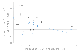
\includegraphics[height=0.3\textheight]{figures/fig-moeng-2.png}
\caption{Average closure duration of those ejectives which have been affricated ([ts’]) decreases as the percent of ejective fricatives with no closure ([s’]) increases (r = -0.54, p = 0.13).}
\label{fig:moeng:3}
\end{figure}

\newpage 
A Pearson Correlation Coefficient of \textit{r} = −0.54 was calculated for the set of points. However, this correlation cannot be said to be significant with a nondirectional \textit{p}{}-value of 0.13. This is due to the maximum sample size of N = 9 that can be derived from a 3x3 environment matrix, not necessarily the robustness of the trend. Performing this same analysis with a larger environment matrix would be the next step in testing the significance of the trend suggested here.

\subsection{Discussion}\label{sec:moeng:5.4}

In order to produce an ejective without complete closure as in the case of ejective fricatives, the loss in air pressure caused by escaping air must be no greater than the rate at which additional pressure is created by compression of the \isi{supralaryngeal cavity}. If this is not attained, then the pressure differential necessary for the production of the ejective burst will be lost. One way to accomplish this would be to “push back” the place of constriction, shrinking the size of the \isi{supralaryngeal cavity} over the course of the segment’s production. Coarticulation with surrounding vowel environments might naturally facilitate or hinder the \isi{movement} of the fricative constriction. 

We thus predict less affrication in vowel contexts where coarticulation causes a backing of the constriction.\footnote{As noted by an anonymous reviewer, we may also expect to see ejectivity preserved more often in “i-i” contexts, due to the narrowness of the palatal constriction. Although this study did not find evidence for this, it would be interesting to further test this idea.} We found that the proportion of un-affricated ejective fricatives was significantly greater following a front vowel [i] and preceding a back vowel [u] (the “i-u” environment) compared to all other vowel environments tested, perhaps due to the \isi{supralaryngeal cavity} being compressed as the fricative articulation transitions out of a front vowel and into a back vowel, counteracting the loss of supralaryngeal pressure from vented air for the fricative. 

This proposal would also predict that when /s’/ \textit{is} produced with closure, the needed duration of that closure in order to create the necessary supralaryngeal pressure would be shorter in an “i-u” environment. Non-significant trends found in Experiment 1 may suggest that this is the case. When there was closure, the average duration of that closure was numerically shortest in the “i-u”, “a-i”, and “a-a” environments. It is possible the “a-i” and “a-a” environments had even shorter average closure durations than that found in the “i-u” environment due to the low vowel [a] forcing the tongue to start from a position vertically distant from the position needed to make the following fricative constriction and thus perhaps causing a shorter duration overall. If this is the case, we perhaps did not also see greater rates of non-affrication in these “a” environments because the greater vertical distance needed to be covered perhaps causes a non-zero (but shorter) closure once the tongue does reach its target destination.

To summarize, although affrication still occurs in the majority of segments in all environments, vowel contexts where coarticulation effects aid regression of the fricative constriction reduce the duration of closure required to create the necessary supralaryngeal pressure. We believe this indicates a dynamic version of Mechanism 4 mentioned earlier, which states that speakers decrease the supralaryngeal volume to produce ejective fricatives (see \sectref{sec:moeng:2.2} and \citealt{demolin2002search}).

Articulation data with high time resolution in a wider variety of vowel contexts would be required to confirm these results. A preliminary ultrasound analysis from one of our participants seems to corroborate Demolin’s findings. \figref{fig:moeng:4} shows average tongue trace contours for the midpoint of an alveolar fricative in \ili{Tigrinya}. Pulmonic /s/ and /z/ are produced with almost identical tongue shapes whereas /s’/ is produced with a backed tongue root, retracting the place of constriction and decreasing the size of the \isi{supralaryngeal cavity}. We should note that these are preliminary findings derived from one speaker with a small stimulus set, and are only taken at the midpoint of the fricative. Therefore, we do not have time-sensitive information regarding the \isi{movement} of the tongue over the course of the fricative in various vowel contexts.

   

\begin{figure}
\includegraphics[height=0.25\textheight]{figures/fig-moeng-3}
\caption{Tongue traces for three alveolar fricatives. Note that the ejective /s’/ (green dashed line) is produced further back than /s/ (red triangles) and /z/ (blue solid).}
\label{fig:moeng:4}
\end{figure}

\section{Experiment 2: Lexical frequency}\label{sec:moeng:6}

The purpose of Experiment 2 is to explore whether \isi{lexical frequency} plays a role in the rate at which /s’/ is produced as an affricate. Various studies have made different claims regarding the role of frequency in variation. For example, \citet{bybee2002word} finds that the rate of \ili{English} coronal stop deletion increases with more frequent words, whereas \citet{labov2011principles} finds that frequency does not play a role in so-called “g”-dropping (e.g. pronouncing \textit{running} as \textit{runnin’}). \citet{hay2015tracking} even finds that low frequency words lead a New Zealand vowel shift. The goal of Experiment 2 is to determine which of these three cases the affrication of /s’/ falls into: (1) no correlation between \isi{lexical frequency} and the affrication of /s’/ (as in “g”-dropping); (2) a positive correlation (as in coronal stop deletion); or (3) a negative correlation (as in the New Zealand vowel shift).

This question is further complicated for an under-resourced language like \ili{Tigrinya}, since there is no traditional corpus from which to obtain lexical frequencies. This experiment will pull from various available sources to attempt to answer this question, but it should be noted that each of these sources has its drawbacks. 

The resource most similar to a traditional corpus that is available for \ili{Tigrinya} is An Crúbadán \citep{scannell2007crubadan}. An Crúbadán is a web-crawler based corpus which aims to provide text corpora for under-resourced languages such as \ili{Tigrinya}. Although a valuable source given the lack of resources available for most of the world’s languages, it is also a small corpus as far as corpora go, with the \ili{Tigrinya} database only containing 1.79 million words from 1291 documents (as compared to 17.9 million words in Celex \citep{BaayenEtAl1993}). In addition, it is primarily based on web documents (e.g. \ili{Tigrinya} Wikipedia, Tweets in \ili{Tigrinya}) which often lack a review process and can thus contain numerous errors. This is in comparison to SUBTLEX which is based on American film subtitles, and to Celex, which draws from a variety of sources (newspapers, books, taped phone conversations, etc). Both of these corpora are also edited and therefore more reliable sources of information compared to the unedited An Crúbadán.

Even with An Crúbadán, there were no entries for the majority of test items, and therefore no information regarding the \isi{lexical frequency} for these items (an indication that the \ili{Tigrinya} corpus from An Crúbadán is too small for our purposes). Therefore, the possibility of using lexical recognition time as a predictor of \isi{lexical frequency} was considered for this study. This is in light of previous studies which have shown that the time it takes to decide whether a string of letters is an actual word or a nonce word is correlated with \isi{lexical frequency} in \ili{German} \citep{brysbaert2011word} and in \ili{English} \citep{baayen2006morphological}. In fact,  \citet{murray2004serial} go so far as to say “[o]f all the possible stimulus variables that might control the time required to recognize a word pattern, it appears that by far the most potent is the frequency of occurrence of the pattern.” 

Words whose frequencies were known from An Crúbadán were included a-mong test stimuli and served as “quality control” items to determine whether the collected reaction times for Experiment 2 were at all indicative of \isi{lexical frequency}. If a strong correlation between recognition time of these items and their frequencies in An Crúbadán were found, this would indicate that recognition time could be used as a rough measure of frequency for those studying under-resourced languages. This would be a valuable tool for linguists working with languages where only small corpora (if any) are available.

Before detailing the methodology of Experiment 2, the authors would like to note that there are a number of complications that greatly affect the interpretability of the results of this experiment, which have been noted by reviewers and other readers of this paper. These will be discussed in \sectref{sec:moeng:6.4} Despite these weaknesses, we felt it was important to still include this experiment here; less for its difficult-to-interpret results, but more to add to the methodological discussion of how linguists might study under-resourced languages, for which the particular piece of information needed to test some theory may not be available. We hope that this experiment will aid future researchers who may also be considering what options may be available to them when certain information is simply not available for a given language.

\subsection{Methodology}\label{sec:moeng:6.1}

Experiment 2 consisted of 2 parts. Part 1 was a Go/No-go word recognition task to determine \isi{lexical frequency} indirectly through reaction times. Part 2 followed Part 1 and consisted of a reading task identical in procedure to that used in Experiment 1.



\subsubsection{Stimuli}\label{sec:moeng:6.1.1}

Stimuli for the Go/No-go task consisted of a mixture of 83 real \ili{Tigrinya} words and 30 viable nonce words, totaling 113 test items. All stimuli words were orthographically represented with three characters in the Ethiopic script, making them either two or three syllables. 

\begin{enumerate}
\item {\textbf{Target Words, word-initial /s’/} \textit{(N=15, e.g.} \amh{ጸሃየ} \textit{/s’ehaje/)}: Actual words in \ili{Tigrinya} which begin with /s’/.}
\item {\textbf{Target Words, word-medial /s’/} \textit{(N=14, e.g.} \amh{ሃጸይ} \textit{/has’ejɨ}\textit{/)}: Actual words in \ili{Tigrinya} which have /s’/ word-medially.}
\item {\textbf{/tʃ’/ Words} \textit{(N=24)}: Actual words with /tʃ’/ word-initially or word-finally. Due to space constraints, these words will not be discussed in the current paper.}
\item {\textbf{Frequency Check Words} \textit{(N=30)}: Actual words in \ili{Tigrinya} for which we have rough frequency estimates for from the small web-crawler corpus, An Crúbadán.}
\item {\textbf{Nonce Words} \textit{(N=30, e.g.} \amh{ራሲካ} \textit{/rasika/)}: Nonwords that are phonotactically-legal in \ili{Tigrinya}.} 
\end{enumerate}

\subsubsection{Procedure}\label{sec:moeng:6.1.2}
\subsubsection{Go/No-go task}\label{sec:moeng:6.1.2.1}

The goal of Part 1 of Experiment 1 was to obtain indirect lexical frequencies via reaction time with a Go/No-go lexical decision task. Stimuli were presented to participants with Psychopy \citep{peirce2007psychopy}. Participants were asked to press the space bar (“go”) only if the string was a real word as quickly as possible. For each trial, the orthographic representation of the stimuli was shown on the screen for a maximum of 3 seconds. If the participant pressed the spacebar on the keyboard or 3 seconds had passed with no response (“no-go”), a black rectangle appeared on the screen for 3 seconds, and the next word would appear. If the spacebar was pressed, the time since the beginning of the trial was recorded. The participants’ view is displayed in \figref{fig:moeng:5}.

   

\begin{figure}
\includegraphics[width=0.9\textwidth]{figures/fig-moeng-4}
\caption{Presentation of stimuli in the Go/No-go task}
\label{fig:moeng:5}
\end{figure}

Participants were first given a demo and instructions in \ili{English}. They were shown actual \ili{English} words (e.g. \textit{find}), as well as nonce words (e.g. \textit{skeep}, \textit{glarp}). Some of the actual words were borrowed words (e.g. \textit{pasta}). For all real words, participants were asked to press the spacebar as quickly as possible, and were told this even applied to words which were borrowed (e.g. \textit{pasta}), but to not press the spacebar if the word was not an actual \ili{English} word. Following the \ili{English} demo, participants were directed to Part 1 of Experiment 2, which was identical in procedure to the \ili{English} demo except words were \ili{Tigrinya} words written in the Ethiopic script. For this portion, participants were given 6 warm-up words which were not included in the analysis, followed immediately by 113 test words, with no break between the warm-up and test trials.

\subsubsection{Production task}\label{sec:moeng:6.1.2.2}

Part 1 was followed by Part 2, in which experimenters recorded participants producing the 29 Target Words. All of these words consisted of the 29 actual words containing /s’/ in Part 1. For the sake of consistency, the procedure in Part 2 was identical to the procedure used in Experiment 1.

\subsection{Analysis}\label{sec:moeng:6.2}

The analysis for Experiment 2 used the same criteria for marking the five landmarks introduced in Experiment 1 (\sectref{sec:moeng:5.2}). As was the case in Experiment 1, if a participant repeated a frame sentence, only the latest repetition was used in the analysis. Word-initial [s’] items were excluded from the analysis if there was a pause before the word, as we would be unable to determine whether there had been a period of closure following the pause.

\subsection{Results}\label{sec:moeng:6.3}

To determine whether any relationship exists between \isi{lexical frequency} and affrication, lexical recognition time and \isi{closure duration} were plotted (\figref{fig:moeng:6}). No correlation was found between reaction time and \isi{closure duration} (\textit{r} = 0.06). This suggests that no relationship exists between affrication and \isi{lexical frequency} as predicted by reaction time.

\begin{figure}
\includegraphics[width=0.8\textwidth]{figures/fig-moeng-5}
\caption{No or very slight negative correlation was found between closure duration and reaction time (r = −0.061).}
\label{fig:moeng:6}
\end{figure}

One goal of this study was also to determine whether lexical recognition time could reliably be used as a predictor of \isi{lexical frequency}, by analyzing the words for which we had a rough measure of frequency from An Crúbadán. The natural logarithm of the frequencies of the Frequency Check words is plotted against participant reaction times in \figref{fig:moeng:7}. A weak but significant correlation (\textit{r} = −0.187, \textit{p} = 0.002) was found between these two variables. For comparison, previous word recognition studies have found correlations between \textit{r} = −0.2 and \textit{r} = −0.4 \citep{brysbaert2011word}, suggesting that our results fell towards the lower bound of correlation values found between \isi{lexical frequency} and reaction times.

   

\begin{figure}
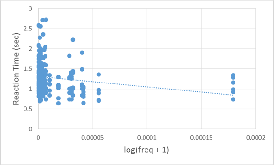
\includegraphics[width=0.8\textwidth]{figures/fig-moeng-6.png}
\caption{Results of the Frequency Check words. Reaction time and lexical frequency are weakly negatively correlated with one another.}
\label{fig:moeng:7}
\end{figure}

\subsection{Discussion}\label{sec:moeng:6.4}

While results of Experiment 2 suggest that there is no correlation between reaction time and \isi{closure duration}, unfortunately due to limitations in language resources, this result could indicate several things. Some weaknesses of Experiment 2 will be discussed here.

Results could simply show that \isi{lexical frequency}, as measured indirectly through a Go/No-go task, is not correlated with \isi{closure duration}. This would place the \isi{closure duration} of an affricated /s’/ with “g”-dropping in \ili{English}, which was also found to have no effect of \isi{lexical frequency} \citep{labov2011principles}.

Frequency Check words had been included to determine whether we were indeed indirectly measuring \isi{lexical frequency}. The frequencies of Frequency Check words showed a very weak correlation with reaction times. With a Pearson’s \textit{r} of only −0.187, any possible correlation might just not be strong enough to use reaction time as an indirect measure of frequency. 

It is also possible that this study did not accurately capture reaction times, either due to flaws in methodology, or due to the small number of participants. For example, the average reaction time among our participants was 1380 ms in contrast to average reaction times between 618–985 ms in other reaction time studies \citep{brysbaert2011word}. It is possible that a difference in the average age of participants played a role here. Whereas past studies with results averaging between 618–985 ms were performed with undergraduate participants presumably between the ages of 18–22, our participants ranged from 20-60 years in age with an average age of 42. Human reaction times have been shown to steadily decrease beginning at the age of 20 \citep{pierson1958movement}, possibly accounting for the difference in reaction time compared with previous studies.

\largerpage
Then again, as noted earlier, An Crúbadán is a small corpus and is only based on words written online. Therefore, An Crúbadán may not even accurately reflect true lexical frequencies in speech, which may be the reason for the low \textit{r} value.

\section{Conclusion}\label{sec:moeng:7}

In Experiment 1, we found that a greater proportion of /s’/ is produced as [s’] when it follows [i] and precedes [u]. We believe this environment naturally facilitates ejective fricatives due to decreasing volume of the \isi{supralaryngeal cavity}. If true, this would further predict that an “i-u” context also aids other ejectives or voiceless phones, and perhaps that the opposite environment “u-i” aids voiced and implosive sounds.

It was hoped for Experiment 2 that indirectly measuring \isi{lexical frequency} with reaction times would give linguists studying under-resourced languages another tool for calculating \isi{lexical frequency}, but multiple weaknesses of Experiment 2 do not allow us to draw any firm conclusions regarding the nature of a possible relationship between affrication and \isi{lexical frequency}, or even regarding the usefulness of using reaction time as an indirect measure of \isi{lexical frequency}. 

\section*{Acknowledgements}

We would like to thank the native speaker consultants for participating in our study and the Eritrean Community Association in Raleigh, NC, as well as David Mora-Marin, Elliott Moreton, Jennifer Smith, and two anonymous reviewers for their helpful comments and suggestions. All errors are of course our own. We would also like to thank Jeff Mielke and the North Carolina State University Phonology Lab for helping us use and allowing us to borrow their ultrasound machine. Special thanks to Ruth Tesfalidet and Tsegga Medhin for helping us choose and create stimuli, and for helping us recruit participants.
 
\largerpage
\sloppy
\printbibliography[heading=subbibliography,notkeyword=this]

\end{document}